%!TEX root = ../thesis.tex

\section{深層学習}

深層学習(Deep learning)は,画像や音声などの複雑なデータを処理するための機械学習手法であり,人工ニューラルネットワークを基盤としている.\figref{Fig:deep_neural_network}に示すように,多層のニューロンが組み合わさり,人間の脳のような階層的な構造をしている.これにより,例えば画像や音声の特徴を学習し,自動的に認識や分類を行うことが可能になる.

\begin{figure}[h]
  \centering
  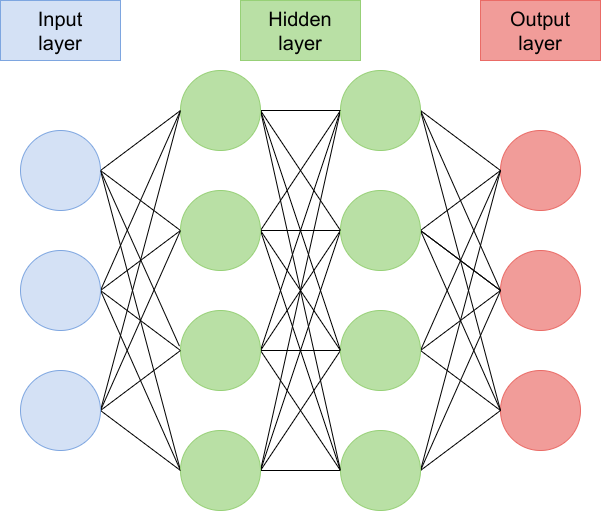
\includegraphics[keepaspectratio, scale=0.30] {images/deep_neural_network.png}
  \caption{Neural network}
  \label{Fig:deep_neural_network}
\end{figure}

\newpage
